\documentclass[en]{../../../eplsummary}

\hypertitle{translators-INGI2132}{8}{3}{4}
{Author}
{Professor}
$$$$

\section{Chapter 1}

\subsection{Compilation}

\subsubsection{Compilers}

A compiler is a program that \textbf{translates} a source program written in
a \textbf{high-level} programming language such as Java, C\# or C, into an
equivalent target program in a \textbf{lower level} language such as machine
code, which can be executed directly by a computer.

\begin{figure}[h]
    \centering
    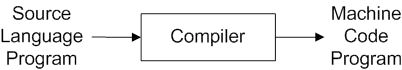
\includegraphics[width=8cm]{img/compilers.png}
    \caption{Compilation}
\end{figure}

\paragraph{Input $\to$ output} 
\begin{itemize}
    \item Mapping names to memory addresses, stack frame offsets and
        registers
    \item Generate linear sequence of machine code instructions
    \item Detecting any errors that can be detected
\end{itemize}


\subsubsection{Interpreters}
Interpreter executed directly th high-level language program.

\begin{figure}[h]
    \centering
    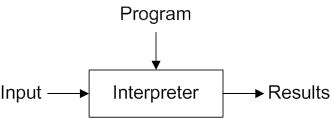
\includegraphics[width=8cm]{img/interpreters.png}
    \caption{Interpretation}
\end{figure}

\begin{enumerate}
    \item \textbf{Performance} : better with compilers (because
        interpreter must parse and analyse the statement ot decode its
        meaning \textit{every time} it execute that statement)
    \item \textbf{Secrecy} : more difficult to understand program with
        machine code
    \item[but] sometime, the overhead of interpretation doesn't always
        justify writing (or buying) a compiler. Like UNIX shell.
\end{enumerate}



\subsubsection{Programming languages}

Specified in three steps :
\begin{enumerate}
    \item \textbf{Tokens} : like work in natural language
    \item \textbf{Syntax}
    \item \textbf{Semantics}
    \item[Note] : The two first are described with formal notation, and
        the last is described with natural language.
\end{enumerate}

\subsubsection{Machines Languages}

A machine language program consists of a sequence of instructions and
operands, usually organized so that each instruction and each operand
occupies one or more bytes and so is easily accessed and interpreted.

A machine instruction set and its behavior is often referred to as its
\textbf{architecture}.

\paragraph{Note:} Java Virtual Machine (JVM) is said \textit{virtual}
because it is not necessarily implemented in hardware, rather it is
implemente as a software.

\subsection{Why study compilers?}




\end{document}
